\documentclass{hw}

\usepackage{minted}

\begin{document}
\noindent\textbf{Talia Hicks, Steven Rosendahl}

\section*{Algorithm 1}

\hspace{-1cm}

\begin{minipage}[t]{0.5\textwidth}

\vspace{-4.5cm}

\begin{minted}[fontsize=\footnotesize,linenos]{java}
public static void algoOne(int[] a){
    int INST_COUT = 0;
    //Begin counting instructions
    int n = a.length;
    int j = 1;
    int[] b = new int[n];
    while(j <= n){
        INST_COUT++;
        int i = 1;
        while(i <= n - j){
            INST_COUT++;
            int m = i + j - 1;
            int r = min(m + j, n);
            int u = i;
            for(; u < r; u++){
                INST_COUT++;
                b[u] = a[u];
            }
            u = i;
            int v = m + 1;
            int w = i;
            for(; w < r; w++){
                INST_COUT++;
                if((u > m) || (v <= r && b[v-1] < b[u-1])){
                    INST_COUT++;
                    a[w] = b[v];
                    v++;
                } else {
                    INST_COUT++;
                    a[w] = b[u];
                    u++;
                }
            }
            i = i + (2 * j);
        }
        j *= 2;
    }
    out.println(INST_COUT);
}
\end{minted}
\end{minipage}
\begin{minipage}[t]{0.5\textwidth}
% \begin{minted}{python}

% \end{minted}
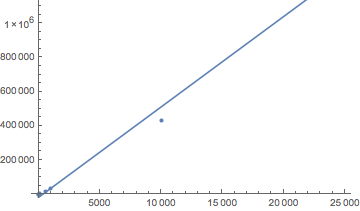
\includegraphics[scale=0.6]{ag1}
\[
\textbf{Runtime: }O(n)
\]
\begin{align*}
&\{5, 29\}, \{10, 97\},\\
&\{55, 1061\}, \{100, 2251\},\\
&\{555, 17321\}, \{1000, 31933\},\\
&\{10000, 428949\}, \{100000, 5278965\}\\
\end{align*}
\end{minipage}

\newpage

\section*{Algorithm 2}

% \begin{minipage}[t]{0.5\textwidth}

\begin{minted}[fontsize=\footnotesize,linenos]{java}
public static void compute(int[] a, int[] b, int i){
    int n = a.length - 1;
    algOps++;
    if(i > n){
        for(int j = 1; j < n; j++){
            algOps++;
            if(b[j] > 0){
                out.println(b[j]);
                algOps++;
            }
        }
        algOps++;
        return;
    }
    b[i] = 0;
    compute(a, b, i + 1);
    b[i] = a[i];
    compute(a, b, i + 1);
    algOps++;
    b[i] = 0;
}
\end{minted}

\vspace{2cm}
\begin{center}
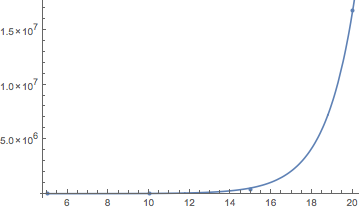
\includegraphics[scale=0.6]{ag2}
\end{center}
\[
\textbf{Runtime: }O(e^x)
\]
\begin{align*}
&\{5, 149\},\\
&\{10, 8701\},\\
&\{15, 401405\},\\
&\{20, 16777213\}\\
\end{align*}
% \end{minipage}
\end{document}
